% Created 2016-06-29 Wed 18:01
\documentclass[11pt]{article}
\usepackage[utf8]{inputenc}
\usepackage[T1]{fontenc}
\usepackage{fixltx2e}
\usepackage{graphicx}
\usepackage{grffile}
\usepackage{longtable}
\usepackage{wrapfig}
\usepackage{rotating}
\usepackage[normalem]{ulem}
\usepackage{amsmath}
\usepackage{textcomp}
\usepackage{amssymb}
\usepackage{capt-of}
\usepackage{hyperref}
\author{Meghana Bandaru}
\date{June 9, 2016}
\title{Document for Docker}
\hypersetup{
 pdfauthor={Meghana Bandaru},
 pdftitle={Document for Docker},
 pdfkeywords={},
 pdfsubject={},
 pdfcreator={Emacs 24.3.1 (Org mode 8.3.4)}, 
 pdflang={English}}
\begin{document}

\maketitle
\tableofcontents


\section{Introduction to Docker}
\label{sec:orgheadline1}
Docker is an open-source technology that that allows you to build, run, test,
and deploy distributed applications inside software containers. It allows you
to package a piece of software in a standardized unit for software development,
containing everything the software needs to run: code, runtime, system tools,
system libraries, etc. Docker enables you to quickly, reliably, and
consistently deploy applications regardless of environment.
You can refer it \href{https://www.docker.com/what-docker#/copy1}{here.}

\section{Benefits of Docker}
\label{sec:orgheadline2}
\begin{description}
\item[{Rapid application deployment}] Containers include the minimal runtime requirements of the application,
reducing their size and allowing them to be deployed quickly.
\end{description}


\begin{description}
\item[{Portability across machines}] An application and all its dependencies can be bundled into a single
container that is independent from the host
version of Linux kernel, platform distribution, or deployment model. This
container can be transfered to another machine that runs Docker, and
executed there without compatibility issues.

\item[{Version control}] You can track successive versions of a container, inspect differences, or roll-back to previous
versions. That means your container can be easily rolled back when required.

\item[{Sharing}] You can use a remote repository to share your container with others.

\item[{Lightweight and minimal overhead}] Docker images are typically very small, which facilitates rapid delivery
and reduces the time to deploy new application containers.

\begin{description}
\item[{Simplified maintenance}] Docker reduces effort and risk of problems with application dependencies.
\end{description}
\end{description}

\section{Docker Architecture}
\label{sec:orgheadline3}
\begin{itemize}
\item Docker uses a client-server architecture
\item The Docker client talks to the Docker daemon, which does the heavy lifting
of building, running, and distributing your Docker containers
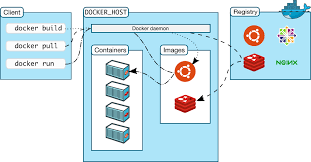
\includegraphics[width=.9\linewidth]{./images/architecture.png}
\end{itemize}
\section{Getting started with Docker}
\label{sec:orgheadline20}
\subsection{Docker images and containers}
\label{sec:orgheadline6}
\begin{description}
\item[{Docker Image}] \begin{itemize}
\item A Docker image is a read-only template.
\item For example, an image could contain an Ubuntu operating system with Apache
and your web application installed.
\item Images are used to create Docker containers.
\item Docker images are the build component of Docker.
\end{itemize}
\item[{Docker Container}] \begin{itemize}
\item A container is a runtime instance of a docker image.
\item Each container is launched from a Docker image.
\item Docker containers can be run, started, stopped, moved, and deleted.
\item Docker containers are the run component of Docker.
\item To use a programming metaphor, if an image is a class, then acontainer is
an instance of a class(a runtime object).
\end{itemize}
\end{description}
\subsubsection{How does Docker images work?}
\label{sec:orgheadline4}
\begin{itemize}
\item Each image consists of a series of layers.
\item Docker makes use of union file systems to combine these layers into a
single image.One of the reasons Docker is so lightweight is because of these
layers.
\item When you change a Docker image-for example, update an application to a new
version, a new layer gets built.
\item Thus, rather than replacing the whole image or entirely rebuilding, only
that layer is added or updated.
\item Now you don't need to distribute a whole new image, just the update,
making distributing Docker images faster and simpler.
\end{itemize}
\subsubsection{How does Docker containers work?}
\label{sec:orgheadline5}
\begin{itemize}
\item A container consists of an operating system, user-added files and
meta-data.
\item The image which we used to create the container tells Docker what that container
holds, what process to run when the container is launched, and a variety
of other configuration data.
\item The Docker image is read-only. When Docker runs a container from an image, it
adds a read-write layer on top of the image in which your application can then run.
\end{itemize}

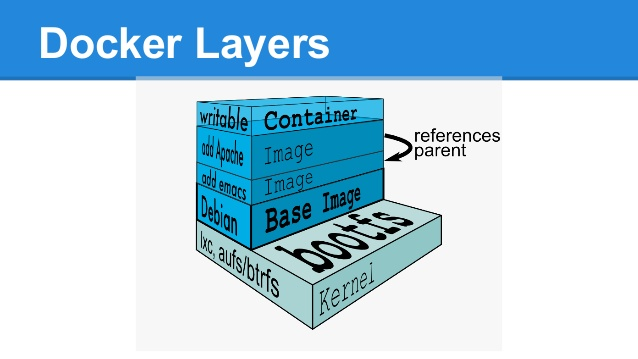
\includegraphics[width=.9\linewidth]{./images/docker-layer.jpg}

\subsection{How to Install docker on Ubuntu 14.04}
\label{sec:orgheadline7}
Installation Instructions on Ubuntu:
\begin{description}
\item[{Update your droplet}] \begin{verbatim}
sudo apt-get update
sudo apt-get -y upgrade
\end{verbatim}
\item[{Make sure aufs support is available}] \begin{verbatim}
sudo apt-get install linux-image-extra-`uname -r`
\end{verbatim}
\item[{Add docker repository key to apt-key for package verification}] \begin{verbatim}
sudo apt-key adv --keyserver hkp://pgp.mit.edu:80 --recv-keys 58118E89F3A912897C070ADBF76221572C52609D
\end{verbatim}
\item[{Add the docker repository to Apt sources}] \begin{verbatim}
echo "deb https://apt.dockerproject.org/repo ubuntu-trusty main" | sudo tee /etc/apt/sources.list.d/docker.list
\end{verbatim}
\item[{Update the repository with the new addition}] \begin{verbatim}
sudo apt-get update
\end{verbatim}
\item[{Finally, download and install docker}] \begin{verbatim}
sudo apt-get install docker-engine
\end{verbatim}
\item[{Check if docker is installed}] \begin{verbatim}
docker version
\end{verbatim}
If you get the following output, then it is successfully installed
\begin{verbatim}
  Client:
  Version:      1.11.2
  API version:  1.23
  Go version:   go1.5.4
  Git commit:   b9f10c9
  Built:        Wed Jun  1 21:47:50 2016
  OS/Arch:      linux/amd64

Server:
 Version:      1.11.2
 API version:  1.23
 Go version:   go1.5.4
 Git commit:   b9f10c9
 Built:        Wed Jun  1 21:47:50 2016
 OS/Arch:      linux/amd64
\end{verbatim}
\end{description}

\subsection{Launch your first container}
\label{sec:orgheadline8}
Launch or execute a command in container using \texttt{docker run} command. This
command will launch a container from an image, execute your command 
display output on terminal, stop container and  exit out.

\begin{verbatim}
docker run-->create container->run-container-->execute command-->show
output-->exit from container-->stop container
\end{verbatim}

\begin{verbatim}
$ sudo docker run [options] [image] [command] [args]
\end{verbatim}
For Example:
\begin{verbatim}
$ sudo docker run ubuntu:14.04 echo "Hello Docker"
$ Hello Docker
\end{verbatim}
If the ubuntu:14.04 image is not present locally it will download it, will
create a container and then will execute the command \texttt{echo}. After this it
will exit the container and the container is stopped.

\subsection{Create/Start/Stop/Restart/Destroy your container}
\label{sec:orgheadline9}
A container is a runtime instance of a docker image.
\begin{description}
\item[{Create a new container}] \begin{verbatim}
docker create [OPTIONS] IMAGE [COMMAND] [ARG...]
\end{verbatim}
For example:
\begin{verbatim}
docker create -it ubuntu:14.04 echo "Hello World"
\end{verbatim}
\begin{itemize}
\item This command can be used to set up a container configuration ahead of time so
\end{itemize}
that it is ready to start when you need it.
\begin{itemize}
\item A container created does not start on it's own and is to be started.
\item Creates a writeable container layer over the specified image.
\end{itemize}

\item[{Start a container}] \begin{verbatim}
docker start [OPTIONS] CONTAINER [CONTAINER...]
\end{verbatim}
For Example:
\begin{verbatim}
$ docker start e76ccff0a41a
e76ccff0a41a
\end{verbatim}
\item[{To stop one or more containers}] \begin{verbatim}
docker stop [OPTIONS] CONTAINER [CONTAINER...]
\end{verbatim}
For Example:
\begin{verbatim}
$ docker stop e76ccff0a41a
e76ccff0a41a
\end{verbatim}

\item[{To restart one or more container}] \begin{verbatim}
docker restart [OPTIONS] CONTAINER [CONTAINER...]
\end{verbatim}
For Example:
\begin{verbatim}
$ docker restart e76ccff0a41a
e76ccff0a41a
\end{verbatim}

\item[{Destroy a container}] \begin{verbatim}
docker rm [OPTIONS] CONTAINER [CONTAINER...]
\end{verbatim}
\begin{itemize}
\item You can destroy one or more containers at a time
\item You cannot delete a container which is currently running. So first stop the
container and then delete it.
\end{itemize}
\begin{verbatim}
$ docker stop e76ccff0a41a
e76ccff0a41a
$ docker rm e76ccff0a41a
e76ccff0a41a
\end{verbatim}
\end{description}

\subsection{Naming a container}
\label{sec:orgheadline10}
\begin{itemize}
\item If you do not specify the name of the container docker will automatically
assume any random name.
\item To give name to a container:
\begin{verbatim}
docker run [options] -name <name of container> <image> <command>
\end{verbatim}
For Example:
\begin{verbatim}
$ docker run -it -name lab1_cse01 ubuntu:14.04 bash
root@8c2fc6ba883b:~#_
\end{verbatim}
\item You can always rename your container
\begin{verbatim}
docker rename [OPTIONS] OLD_NAME NEW_NAME
\end{verbatim}
For Example:
\begin{verbatim}
$ docker rename lab1_cae01 lab2_cse02
\end{verbatim}
\end{itemize}

\subsection{Giving a hostname to container}
\label{sec:orgheadline11}
\begin{itemize}
\item To give host name to container you must use \texttt{-h} flag with the \texttt{docker run} command:
\begin{verbatim}
docker run -h <hostname> [options] [image] [command]
\end{verbatim}
For Example:
\begin{verbatim}
$ docker run -h new_ctnd -it ubuntu:14.04 bash
root@new_cntd:~#_
\end{verbatim}
\end{itemize}
\subsection{List container}
\label{sec:orgheadline12}
\texttt{docker ps} command is used to list containers in host machine. Depending on
the flags provided, it displays information of stopped or running containers.  
\begin{verbatim}
docker ps [options]
\end{verbatim}

\begin{description}
\item[{List the containers which are currently running}] \begin{verbatim}
$ docker ps
CONTAINER ID    IMAGE          COMMAND    CREATED              STATUS              PORTS           NAMES
07c5614d5a40    ubuntu:14.04   "bash"     About a minute ago   Up About a minute                   evil_fermi
e76ccff0a41a    ubuntu:14.04   "bash"     4 days ago           Up 12 minutes                       stoic_bhabha
\end{verbatim}

\item[{List all the containers(both running and stopped)}] \begin{verbatim}
$ docker ps -a
CONTAINER ID        IMAGE                    COMMAND             CREATED             STATUS                    PORTS               NAMES
07c5614d5a40        ubuntu:14.04             "bash"              5 minutes ago       Up 5 minutes                                  evil_fermi
e76ccff0a41a        ubuntu:14.04             "bash"              4 days ago          Up 15 minutes                                 stoic_bhabha
ca251b8c44d8        ubuntu:14.04             "bash"              4 days ago          Exited (0) 4 days ago                         sad_wright
58d28030aa5e        ubuntu:14.04             "bash"              4 days ago          Exited (0) 4 days ago                         jolly_raman
34ab6efd089f        lab/problem-solving:01   "bash"              5 days ago          Exited (0) 4 days ago                         insane_yalow
4164528c53c3        ubuntu:14.04             "bash"              5 days ago          Exited (0) 4 days ago                         pensive_hypatia
ec164228902a        ubuntu:14.04             "bash"              5 days ago          Exited (0) 21 hours ago                       tiny_aryabhata
8c2fc6ba883b        ubuntu:14.04             "bash"              5 days ago          Exited (0) 30 hours ago                       new-name
\end{verbatim}
OR
\begin{verbatim}
$ docker ps -as
CONTAINER ID        IMAGE                    COMMAND             CREATED             STATUS                    PORTS               NAMES               SIZE
07c5614d5a40        ubuntu:14.04             "bash"              6 minutes ago       Up 6 minutes                                  evil_fermi          0 B (virtual 188 MB)
e76ccff0a41a        ubuntu:14.04             "bash"              4 days ago          Up 17 minutes                                 stoic_bhabha        164 B (virtual 188 MB)
ca251b8c44d8        ubuntu:14.04             "bash"              4 days ago          Exited (0) 4 days ago                         sad_wright          203.8 kB (virtual 188.2 MB)
58d28030aa5e        ubuntu:14.04             "bash"              4 days ago          Exited (0) 4 days ago                         jolly_raman         63.87 MB (virtual 251.8 MB)
34ab6efd089f        lab/problem-solving:01   "bash"              5 days ago          Exited (0) 4 days ago                         insane_yalow        1.385 MB (virtual 788.7 MB)
4164528c53c3        ubuntu:14.04             "bash"              5 days ago          Exited (0) 4 days ago                         pensive_hypatia     153.1 MB (virtual 341.1 MB)
ec164228902a        ubuntu:14.04             "bash"              5 days ago          Exited (0) 21 hours ago                       tiny_aryabhata      1.25 GB (virtual 1.438 GB)
8c2fc6ba883b        ubuntu:14.04             "bash"              5 days ago          Exited (0) 30 hours ago                       new-name            0 B (virtual 188 MB)
\end{verbatim}
\begin{itemize}
\item flag \texttt{a} for all containers
\item flag \texttt{s} for size of containers
\end{itemize}
\end{description}

\subsection{List images}
\label{sec:orgheadline13}
List all the images currently sitting in your local repository/system
\begin{verbatim}
$ docker images
REPOSITORY            TAG                 IMAGE ID            CREATED             SIZE
labs/speech-recog     latest              1e85be4efa89        5 days ago          341.1 MB
lab/problem-solving   01                  be7d953b67e6        5 days ago          787.3 MB
meghanab/myapp        1.0                 08570d8b4a10        13 days ago         267.3 MB
meghana/new_image1    0.1                 2934249749c9        2 weeks ago         252.9 MB
meghana/new_user      1                   b5900443b2d7        2 weeks ago         188.3 MB
centos                7                   904d6c400333        3 weeks ago         196.8 MB
ubuntu                14.04               8f1bd21bd25c        4 weeks ago         188 MB
\end{verbatim}
\subsection{List processes running inside a container}
\label{sec:orgheadline14}
\begin{description}
\item[{Display the running processes of a container}] \begin{verbatim}
$ docker top [container]
\end{verbatim}
For Example:
\begin{verbatim}
$ docker top ec164228902a
UID            PID             PPID           C              STIME           TTY            TIME             CMD
root           5207            5192           0              20:32           pts/9          00:00:00         bash
\end{verbatim}
\end{description}

\subsection{Running your container in detached mode}
\label{sec:orgheadline15}
\begin{verbatim}
docker run -d [image] [command]
\end{verbatim}
\begin{itemize}
\item This will run the command in the background and will automatically shuts down
the container after its execution
\end{itemize}

For Example:
\begin{verbatim}
$ docker run -d ubuntu:14.04 bash
698de53f5f4b151122e18b51d4abb813b4e1dff10e30472791dd5ec336fb4b10
$
\end{verbatim}
\subsection{Execute a command inside a container from host machine}
\label{sec:orgheadline16}
\begin{itemize}
\item You can execute a command inside a container from the host machine
provided the container is in running state. Othrewise you have to start
the container first and then use the following command
\end{itemize}
\begin{verbatim}
docker exec [OPTIONS] CONTAINER COMMAND [ARG...]
\end{verbatim}
FOr example:
\begin{verbatim}
root@meghana / $ docker ps
CONTAINER ID   IMAGE          COMMAND      CREATED        STATUS              PORTS               NAMES
e76ccff0a41a   ubuntu:14.04   "bash"       2 days ago     Up About an hour                        stoic_bhabha

root@meghana / $ docker exec e76ccff0a41a ping 127.0.0.1 -c 5
PING 127.0.0.1 (127.0.0.1) 56(84) bytes of data.
64 bytes from 127.0.0.1: icmp_seq=1 ttl=64 time=0.050 ms
64 bytes from 127.0.0.1: icmp_seq=2 ttl=64 time=0.053 ms
64 bytes from 127.0.0.1: icmp_seq=3 ttl=64 time=0.055 ms
64 bytes from 127.0.0.1: icmp_seq=4 ttl=64 time=0.033 ms
64 bytes from 127.0.0.1: icmp_seq=5 ttl=64 time=0.054 ms

--- 127.0.0.1 ping statistics ---
5 packets transmitted, 5 received, 0% packet loss, time 3997ms
rtt min/avg/max/mdev = 0.033/0.049/0.055/0.008 ms
\end{verbatim}

\begin{itemize}
\item You can use various flags with this command
\end{itemize}
\begin{verbatim}
  -d, --detach               Detached mode: run command in the background
  -i, --interactive          Keep STDIN open even if not attached
  -t                         Allocate a pseudo Terminal
\end{verbatim}
\subsection{Get inside a container}
\label{sec:orgheadline17}
To get terminal access to container you need to fire some commands. This may be
required to install packages and configure them inside your container.
\begin{description}
\item[{Case 1}] If you want to enter into a container as soon as you create it:
\begin{verbatim}
docker run -it <repository>:<tag> bash
\end{verbatim}
\begin{itemize}
\item -i flag to connect STDIN on the container
\item -t flag to get a pseudo terminal
\end{itemize}
+For Example:
\begin{verbatim}
$ docker run -it ubuntua:14.04 bash
root@ec164228902a:~#
\end{verbatim}

\item[{Case 2}] If you fire \texttt{bash} command inside a container, it runs forever, until
manually stopped. By giving -d flag to \texttt{docker run}  a container executes
and runs in detached mode, with no interaction with user. So to get inside a
container which is running in detached mode:
\begin{description}
\item[{Method 1}] Using exec command
\begin{verbatim}
docker exec -it <Container ID> bash
\end{verbatim}
For Example:
\begin{verbatim}
$ docker exec -it ec164228902a bash
root@ec164228902a:~#
\end{verbatim}
\begin{description}
\item[{To come out of the container without stopping it}] 
\end{description}
\begin{verbatim}
CTRL+P+Q
\end{verbatim}
OR
\begin{verbatim}
exit
\end{verbatim}
\begin{verbatim}
root@ec164228902a:~# exit
root@meghana ~ $
root@meghana ~ $ docker ps
CONTAINER ID        IMAGE               COMMAND             CREATED             STATUS              PORTS               NAMES
07c5614d5a40        ubuntu:14.04        "bash"              21 minutes ago      Up 21 minutes                           evil_fermi
ec164228902a        ubuntu:14.04        "bash"              4 days ago          Up 32 minutes                           stoic_bhabha
\end{verbatim}

\item[{Method 2}] Using Attach command
\begin{verbatim}
docker attach <Container ID>
\end{verbatim}
\begin{itemize}
\item You might need to hit Enter to bring up the prompt.
\end{itemize}
For Example:
\begin{verbatim}
$ docker attach ec164228902
$
root@ec164228902:~#
\end{verbatim}
\begin{description}
\item[{To get out of the container without stopping it}] 
\end{description}
\begin{verbatim}
CTRL+P+Q
\end{verbatim}
\end{description}
\end{description}

\subsection{Auto restart Containers}
\label{sec:orgheadline18}
If your host machine shuts down, all container will be stopped. Once your
restart your machine, all container should automatically start. To add such
behavior to all your containers, you need to add a flag \texttt{-{}-restart} in
\texttt{docker run} command. 
\begin{verbatim}
docker run [options] --restart=always [image] [command]
\end{verbatim}
For Example:
\begin{verbatim}
$ docker run -d -it --restart=always meghanab/app1:0.1 bash
\end{verbatim}
\begin{itemize}
\item We need to specify whether you want to auto-start your container at the
time of its creation itself.
\end{itemize}

\subsection{Some Important flags with \texttt{docker run} command}
\label{sec:orgheadline19}
\begin{itemize}
\item \texttt{-i}  connect STDIN on the container
\item \texttt{-t}  Give pseudo Terminal to the container
\item \texttt{-d}  Run the container in detached mode
\item \texttt{-p}  To specify ports or range of ports
\item \texttt{-c}  Limit CPU shares
\item \texttt{-m}  Memory limit
\end{itemize}
\begin{verbatim}
$ docker run -i -t -d -p 80:80 -c 10 -m 300M ubuntu:14.04 bash
\end{verbatim}
\section{Advanced operations in Docker}
\label{sec:orgheadline37}
\subsection{Create an image from your container}
\label{sec:orgheadline21}
One can commit a container and can create its image. Thus we can save the state
a container. This image can be used to launch new container with all the
packages installed hence replicating the state of the container. This helps
in creating a reusable image for launching multiple containers with
customized applications of your need. 

\begin{verbatim}
docker commit <container ID> <Repository>:<tag>
#For Example:
$ docker commit ec164228902 meghanab/myapp:1.0
sha256:4069d3511b08f810c6b725f64360f10148a46a8e5f66a111304585e33af1e912
\end{verbatim}

\subsection{Dockerfile}
\label{sec:orgheadline23}
A Dockerfile is a text document that contains all the commands you would
normally execute manually in order to build a Docker image. Docker can build
images automatically by reading the instructions from a Dockerfile.
\begin{itemize}
\item Thus we can say that Dockerfike is a configuration file used to build docker images
\item It is more effective and easier way compared to \texttt{docker commit}
\end{itemize}
\begin{description}
\item[{Writing Dockerfile}] \begin{itemize}
\item Docker file instructions
\begin{itemize}
\item \texttt{FROM}: for specifying the base image
\item \texttt{RUN}: for specifying commands to execute
\end{itemize}
\begin{verbatim}
$ vim Dockerfile 
#Example of a Docker File
FROM ubuntu:14.04
RUN apt-get install -y  vim
RUN apt-get insatll -y curl
\end{verbatim}

OR

\begin{verbatim}
#Just another way of Docker File
$ vim Dockefile
FROM ubuntu:14.04
RUN apt-get update && apt-get install -y vim \
                                    curl
\end{verbatim}
\item The second method of dockerfile is more preferable as in first case for each run
command an intermediate container gets created and destroyed where as in
second method only one intermediate container will get created and destroyed
\begin{itemize}
\item Thus Second method is more preferable.
\end{itemize}
\end{itemize}
\item[{Building a image from our Docker File}] \begin{verbatim}
docker build -t [repository]:[tag] [path]
\end{verbatim}
\begin{itemize}
\item Now you can use this image \texttt{[repository]:[tag]} to create containers
\end{itemize}
For Example:
\begin{verbatim}
docker build -t meghanab/new_app:1.0 .
\end{verbatim}
\begin{itemize}
\item \texttt{-t} for specifying the image tag
\item \texttt{.} to specify the path of Dockerfile. In this case it is in the current directory
\end{itemize}
\item[{Launching a container from our new image}] \begin{verbatim}
docker run [options] [repository]:[tag] [command]
\end{verbatim}
For Example:
\begin{verbatim}
$ docker run -it -d meghanab/new_app:1.0 bash
root@e76ccff0a41a:~#
\end{verbatim}
\begin{itemize}
\item Thus a new container will be created and started with vim and curl pre
installed. Similarly we can install other packages.
\end{itemize}
\end{description}
\subsubsection{Some more info on Dockerfile}
\label{sec:orgheadline22}
\begin{description}
\item[{CMD Instruction}] \begin{itemize}
\item defines a default command that will execute when the container is
created/started whose base image is built using dockerfile
\item will not perform any action when the image is being created
\item can only be specified once in a dockerfile
\item can be overriden at run time
\end{itemize}
For eg:
\begin{verbatim}
FROM ubuntu:14.04
RUN apt-get update && apt-get install -y vim \
                                   curl
CMD ping 127.0.0.1 -c 10
\end{verbatim}
\item[{ENTRYPOINT instruction}] \begin{itemize}
\item Defines the command that will run when the container is executed
\item Differnt from \texttt{CMD} instruction as \texttt{ENTRYPOINT} instruction will accept
arguments at run time
\end{itemize}
\begin{verbatim}
ENTRYPOINT ["executable", "param1", "param2"]
\end{verbatim}
For eg:
\begin{verbatim}
FROM ubuntu:14.04
RUN apt-get update && apt-get install -y vim \
                                    curl
ENTRYPOINT ["ping"]
\end{verbatim}
\begin{itemize}
\item Only the last \texttt{ENTRYPOINT} instruction in the Dockerfile will have an effect.
\item The \texttt{ENTRYPOINT} instruction is given in exec form which will take
parameters in json format as it has to accept args at run time
\item \texttt{CMD} instruction can also be given in exec format
\item You can give only one command in the \texttt{ENTRYPOINT} instruction
\end{itemize}
\begin{verbatim}
docker run <repository>:<tag> 127.0.0.1
\end{verbatim}

\item EXPOSE
The \texttt{EXPOSE} command is used to associate a specified port to enable networking
between the running process inside the container and the outside world
(i.e. the host).
Example:
\begin{verbatim}
# Usage: EXPOSE [port]
EXPOSE 8080EXPOSE
\end{verbatim}
\item ADD
The \texttt{ADD} instruction copies new files, directories or remote file URLs
from <src> and adds them to the filesystem of the container at the path
<dest>.
\begin{verbatim}
$ ADD <src>... <dest>
OR   
$ ADD ["<src>",... "<dest>"] (this form is required for paths containing whitespace)
\end{verbatim}
\end{description}

\subsection{Run a container as a server}
\label{sec:orgheadline25}
\begin{itemize}
\item We can run a container as long as you don't kill the process with PID 1
\item If a process with PID 1 is killed inside a container then the container will
automatically stop.
\item In the \texttt{docker run [options] [image] [command]}, the command which you give
will become the process with PID 1
\item If we give "bash" as command then the container will not stop until we
manually kill bash process in that container.
\end{itemize}
\subsubsection{Steps to set up a container as a server}
\label{sec:orgheadline24}
\begin{description}
\item[{Create and run a container}] \begin{verbatim}
docker run [options] [image] [command]
\end{verbatim}
\begin{itemize}
\item So let us give bash command
\end{itemize}
\begin{verbatim}
docker run -i -t ubuntu:14.04 bash
\end{verbatim}
\begin{itemize}
\item This command will create a new container and will take us inside the
\end{itemize}
container
\begin{itemize}
\item Now if you fire \texttt{ps -ax} you can see the bash process with PID 1
\end{itemize}
\begin{verbatim}
PID TTY      STAT   TIME COMMAND
  1 ?        Ss+    0:00 bash
 51 ?        R+     0:00 ps -ax
\end{verbatim}
\begin{itemize}
\item So now if you fire \texttt{exit} you will kill the process bash and you will come out of the container and the
container stops, which is not desired.
\item If you want to come out of the container and keep it running in background,
then fire:
\begin{verbatim}
CTRL+P+Q
\end{verbatim}
\item If the host system is rebooted then this container is stopped. So to avoid
this we have to give \texttt{-{}-restart=always} flag at the time of creating container. It is
explained in the following section.
\end{itemize}
\end{description}
\subsection{To view the Docker containers resource usage statistics}
\label{sec:orgheadline26}
\begin{verbatim}
docker stats --no-stream=true
\end{verbatim}
For Example:
\begin{verbatim}
$ docker stats --no-stream=true
CONTAINER           CPU %               MEM USAGE / LIMIT     MEM %               NET I/O             BLOCK I/O           PIDS
07c5614d5a40        0.00%               544.8 kB / 4.064 GB   0.01%               5.245 kB / 648 B    0 B / 0 B           0
e76ccff0a41a        0.00%               532.5 kB / 4.064 GB   0.01%               6.214 kB / 648 B    0 B / 0 B           0
\end{verbatim}
\subsection{Docker Data Volumes}
\label{sec:orgheadline33}
\begin{itemize}
\item Data volumes are designed to persist data.
\item These are independent of the container's life cycle i.e even though
containers are deleted volumes persist.
\item Volumes are initialized when a container is created.
\item Data volumes can be shared and reused among containers.
\item Changes to a data volume will not be included when you update an image.
\end{itemize}
\subsubsection{Create Volume}
\label{sec:orgheadline27}
\begin{itemize}
\item To create anew volume
\begin{verbatim}
docker volume create [OPTIONS]
\end{verbatim}
-You can create a volume and then configure the container to use it, for example:
\begin{verbatim}
docker volume create --name hello
docker run -d -v hello:/world <image> <command>
\end{verbatim}
\begin{itemize}
\item Here the mount is created inside the container's /world directory.
\end{itemize}
\end{itemize}
\subsubsection{Mount Host Directory}
\label{sec:orgheadline28}
To mount a directory from host to your container
\begin{verbatim}
docker run [options] -v /<host_dir>:/<container_dir> [image] [command]
\end{verbatim}
For Example:
\begin{verbatim}
docker run -it -v /home/meghana/project:/test ubuntu:14.04 bash
\end{verbatim}
\begin{itemize}
\item This command mounts the host directory, /home/meghana/project, into the
container at /test
\item All the files in /home/meghana/project can accessed from /test inside the
container
\end{itemize}
\subsubsection{Inspect}
\label{sec:orgheadline29}
\begin{itemize}
\item To get information about one or more volumes
\begin{verbatim}
docker volume inspect [OPTIONS] VOLUME [VOLUME...]
\end{verbatim}
For example:
\begin{verbatim}
docker volume create --name volume_1
\end{verbatim}
\begin{verbatim}
docker volume inspect volume_1
[
  {
     "Name": "volume_1",
     "Driver": "local",
     "Mountpoint": "/var/lib/docker/volumes/volume_1/_data",
     "Labels": {}
  }
]
\end{verbatim}
\end{itemize}
\subsubsection{Delete Volume}
\label{sec:orgheadline30}
\begin{itemize}
\item To delete one or more volumes
\begin{verbatim}
docker volume rm [OPTIONS] VOLUME [VOLUME...]
\end{verbatim}
\begin{itemize}
\item You cannot remove a volume that is in use by a container.
\end{itemize}
\end{itemize}
\subsubsection{List Volumes}
\label{sec:orgheadline31}
\begin{itemize}
\item To list all the volumes present
\begin{verbatim}
docker volume ls [OPTIONS]
\end{verbatim}
\begin{verbatim}
DRIVER              VOLUME NAME
local               volume_1
local               volume_2
\end{verbatim}
\end{itemize}
\subsubsection{Note:}
\label{sec:orgheadline32}
We added a new data-volume
\begin{verbatim}
docker run -it -v hello:/test ubuntu:14.04 bash
\end{verbatim}
We tried to copy a file of 20GB from host machine to container using SCP
\begin{verbatim}
scp -r meghana@10.2.59.17:/media .
\end{verbatim}
But it was not able to copy more than 9GB after that it shows dick space
exeeded.
So we mounted the host directory to the contaier successfully and we are
able to access those files from container
\subsection{Taking backup of Docker Containers and images}
\label{sec:orgheadline36}
\subsubsection{Backup Docker Images}
\label{sec:orgheadline34}
\begin{itemize}
\item Save the Docker Image
\begin{verbatim}
docker save -o <name_of_backup.tar> <image>
\end{verbatim}
For Example:
\begin{verbatim}
$ docker save -o bkb_image1.tar image1
\end{verbatim}
\begin{itemize}
\item This tar file will be stored in your current directory
\end{itemize}

\item Load the backup image
\begin{verbatim}
docker load -i <name_of_backup.tar>
\end{verbatim}
For Example:
\begin{verbatim}
$ docker load -i bkb_image1.tarx
\end{verbatim}
\begin{itemize}
\item If you run \texttt{docker images} you can see your image
\end{itemize}
\end{itemize}
\subsubsection{Backup Docker Containers}
\label{sec:orgheadline35}
\begin{itemize}
\item Export docker containers
\begin{verbatim}
docker export -o <backup_file_name.tar> <container ID>
\end{verbatim}
For Example:
\begin{verbatim}
$ docker export -o bkb_cntd1.tar 07c5614d5a40
\end{verbatim}
\begin{itemize}
\item Exports the contents of a container's filesystem as a tar archive
\item The \texttt{docker export} command does not export the contents of volumes
associated with the container.
\end{itemize}

\item Import docker containers
\begin{verbatim}
docker import <backup_file_name.tar>
\end{verbatim}
For Example:
\begin{verbatim}
$ docker import bkb_cntd1.tar
\end{verbatim}
\begin{itemize}
\item This command will create a new image and then using that image you have
to create your container
\end{itemize}
\end{itemize}

\section{Docker Hub}
\label{sec:orgheadline44}
\subsection{what is a Docker hub?}
\label{sec:orgheadline38}
The Docker Hub is a public registry maintained by Docker, Inc. It contains
images you can download and use to build containers. It also provides
authentication, work group structure, workflow tools like webhooks and build
triggers, and privacy tools like private repositories for storing images you
don't want to share publicly.
You can refer \href{https://docs.docker.com/docker-hub/}{here}
\subsection{How to use Docker hub?}
\label{sec:orgheadline43}
\subsubsection{Account creation and login}
\label{sec:orgheadline39}
\begin{itemize}
\item create a Docker ID(You can do this through  \href{https://hub.docker.com/}{Docker Hub})
\item Once you have a Docker ID, log into your account from the command line
\end{itemize}
\begin{verbatim}
docker login
Login with your Docker ID to push and pull images from Docker Hub. If you don't have a Docker ID, head over to https://hub.docker.com to create one.
Username: 
Password: 
Login Succeeded
\end{verbatim}
\begin{itemize}
\item Once you have logged in from the command line, you can commit and push to
interact with your repos on Docker Hub.
\end{itemize}
\subsubsection{Search for images}
\label{sec:orgheadline40}
You can search the Docker Hub registry via its search interface or by using the
command line interface:
\begin{verbatim}
docker search [image]
\end{verbatim}
\subsubsection{Pull images}
\label{sec:orgheadline41}
Once you've found the image you want, you can download it with
\begin{verbatim}
docker pull <imagename>:
\end{verbatim}
\subsubsection{Push images}
\label{sec:orgheadline42}
In order to push an image int your docker hub the name of the image
should be same as that of the repository in your docker hub account. 
\begin{verbatim}
$ docker push yourname/newimage
\end{verbatim}
The image will then be uploaded and available for use by your team-mates and/or
the community.You can also make the repository private.
For more info refer this \href{https://docs.docker.com/engine/userguide/containers/dockerrepos/}{link}
\section{Performance Testing}
\label{sec:orgheadline50}
\begin{itemize}
\item We trird to analyse the performance of Docker containers by giving load on
197 Docker containers(each container deployed with one lab) using the
following methods:
\end{itemize}
\subsection{Test using curl command and crontab}
\label{sec:orgheadline45}
Curl is a tool to transfer data from or to a server, using one of the
protocol HTTP, HTTPS out of many supported protocols. Using this feature of
curl command, we tried generating load on containers. Here are the steps -

\begin{description}
\item[{1. Write a script to send 10000 curl request to a container}] \begin{verbatim}
root@vlead-pc:~/load-scripts# vim load-test-script.sh
\end{verbatim}

\begin{verbatim}
#!/bin/sh

echo "START TEST : `date`"
a=0
count=0
while [ $a -lt 10000 ]
do
      curl http://$1
      a=`expr $a + 1`
      count=`expr $count + 1`
done
\end{verbatim}
\item[{2. Write a script to generate crontab entries for executing load-testing script for all containers}] \begin{verbatim}
root@vlead-pc:~/load-scripts# vim create-crontab.sh
\end{verbatim}
\begin{verbatim}
#!/bin/sh

a=2
ip="172.17.0."
file=">/root/load-scripts/data"
while [ $a -lt 200 ]
do
    echo  $1 $2 $ip$a $file$a
    a=`expr $a + 1`
done
\end{verbatim}
\item[{3. Copy paste the ouput of above script in crontab}] \begin{verbatim}
crontab -e
\end{verbatim}

\item[{4. Write a script to check the \texttt{docker stats}}] \begin{verbatim}
root@vlead-pc:~/load-scripts# cat get-stat.sh
\end{verbatim}

\begin{verbatim}
#!/bin/sh

a=0
while [ $a -lt 100 ]
do
    echo "`docker stats --no-stream=true`"
    a=1
    echo ""
done
\end{verbatim}
\item[{5. Write a script to analyse output of docker stats}] \begin{verbatim}
#!/bin/sh

cat $1 | awk '{print $2}' | sed 's/%//g' | sed '/CPU/d' | sed '/^$/d' > ouput.txt
split -l 197 ouput.txt
for i in `find x*`
do
   echo "`awk '{ sum += $1 } END { print sum }' $i`"
done
\end{verbatim}
\item[{6. Following graphs were obtained}] 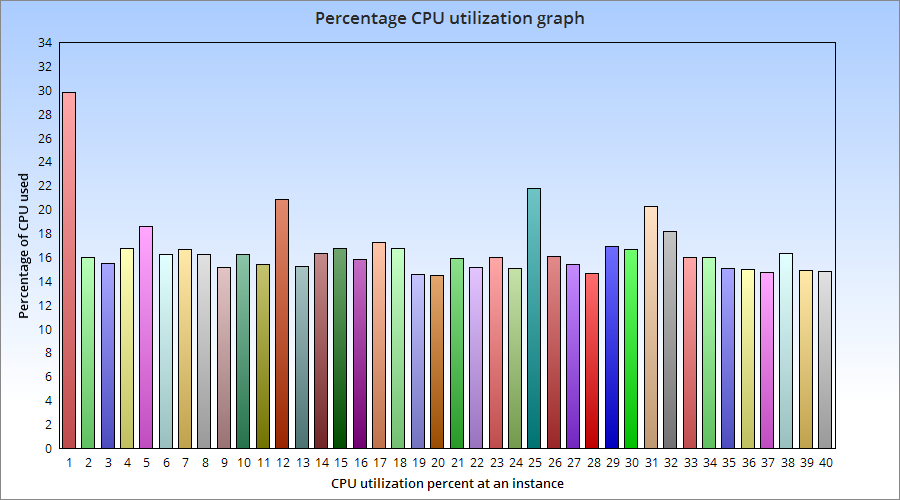
\includegraphics[width=.9\linewidth]{./images/CPU-utilization-bar-graph.png}
   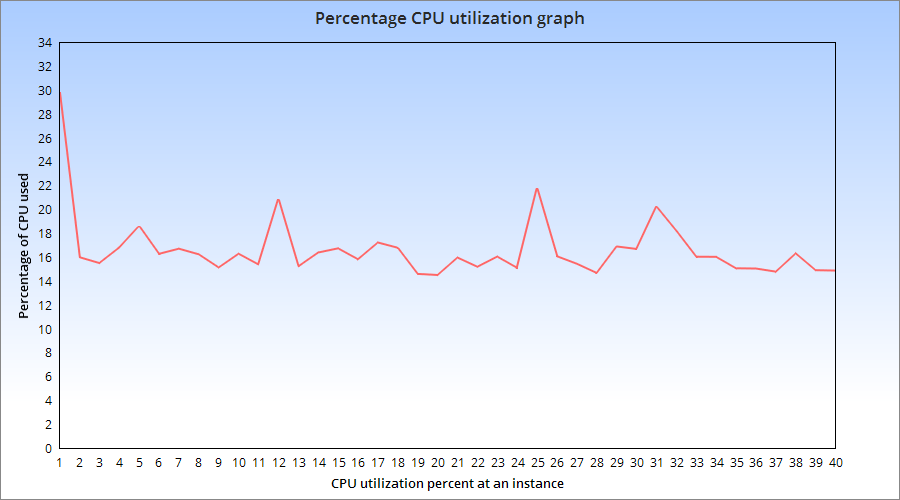
\includegraphics[width=.9\linewidth]{./images/CPU-utilizaton-line-graph.png}
   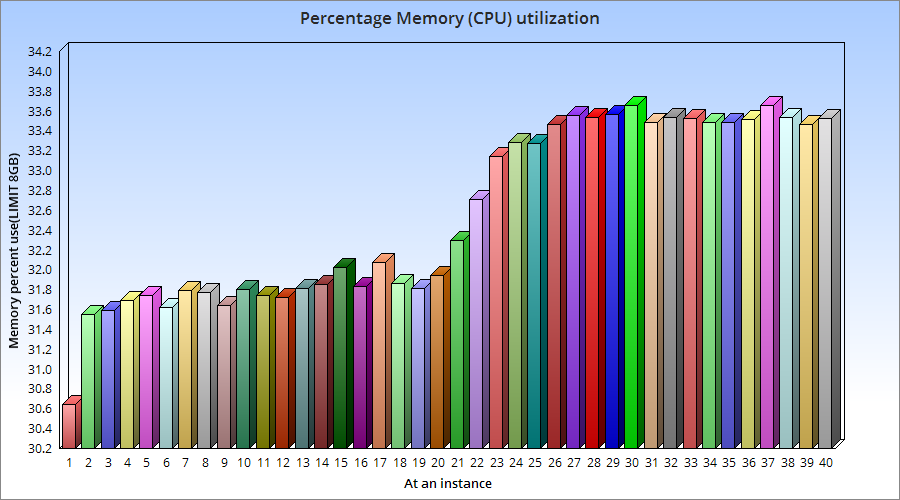
\includegraphics[width=.9\linewidth]{./images/memory-utilization-bar-graph.png}
   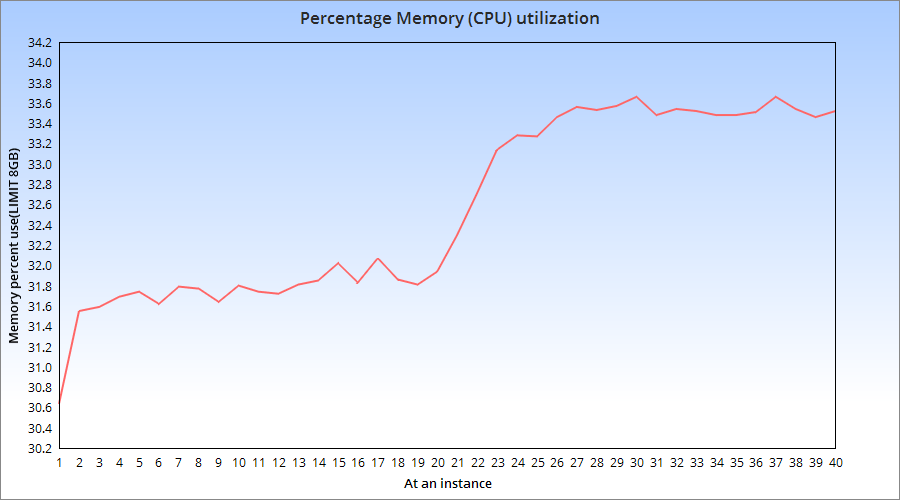
\includegraphics[width=.9\linewidth]{./images/memory-utilization-line-graph.png}
\end{description}
\subsection{Test using siege and sar commands}
\label{sec:orgheadline46}
\begin{itemize}
\item Siege is an HTTP load testing and benchmarking utility that can be used to
measure the performance of a web server when under duress. It evaluates the
amount of data transferred, response time of the server, transaction rate,
throughput, concurrency, and times the program returned okay
\item sar command is used to collect, report, or save system activity information.
\item Using the \texttt{siege} command we tried to generate load on the
containers.Following are the steps:

\item[{1.Install sar,siege and configure them}] To install sar refer \href{http://www.vishalvyas.com/2012/05/installing-system-activity-reporter-sar.html}{here}.
To install siege refer \href{https://www.linode.com/docs/tools-reference/tools/load-testing-with-siege}{here}.
\item[{2.Use sar command to get the memory(RAM) usage statistics when the Containes are}] \begin{itemize}
\item Stopped
\item Started
\item Containers were running
\item Apache is started in containers
\item Apache is running in containers
\end{itemize}
\begin{verbatim}
sar -r 5 10
\end{verbatim}
\begin{itemize}
\item Redirect the output to a file in each case
\end{itemize}
\item[{4. Write a script to generate siege commands}] \begin{verbatim}
root@vlead-pc:~/load-scripts# vim generate-siege-file.sh
\end{verbatim}
\begin{verbatim}
#!/bin/sh

a=2
while [ $a -lt 200 ]
do
   echo "siege -c $1 -t $2s http://172.17.0.$a &"
   echo 'echo "SEIGE CONTAINER $a"'
   a=`expr $a + 1`
done
\end{verbatim}
\begin{itemize}
\item Running this script will generate siege commands for all the containers
\end{itemize}
\item[{5.Copy these siege commands to siege-test.sh}] \begin{verbatim}
sh generate-siege-file.sh [no. of users] [Total time] > siege-test.sh
\end{verbatim}
\item 6.Run \texttt{sar -r [time interval] [no of times]} and \texttt{sh siege-test.sh}
  parallely and redirect the output of \texttt{sar} command to output.txt
\item 7.Change the values of 'no of users' and 'total time' in step 7 and repeat
step 8 for each set of values and redirect the output of \texttt{sar} command to
output.txt
\item 8.Take the values of 'Time' and '\%mem used' from output file and depict
graphs. You can view the data \href{./sar-test.org}{here}

The following graphs were obtained:
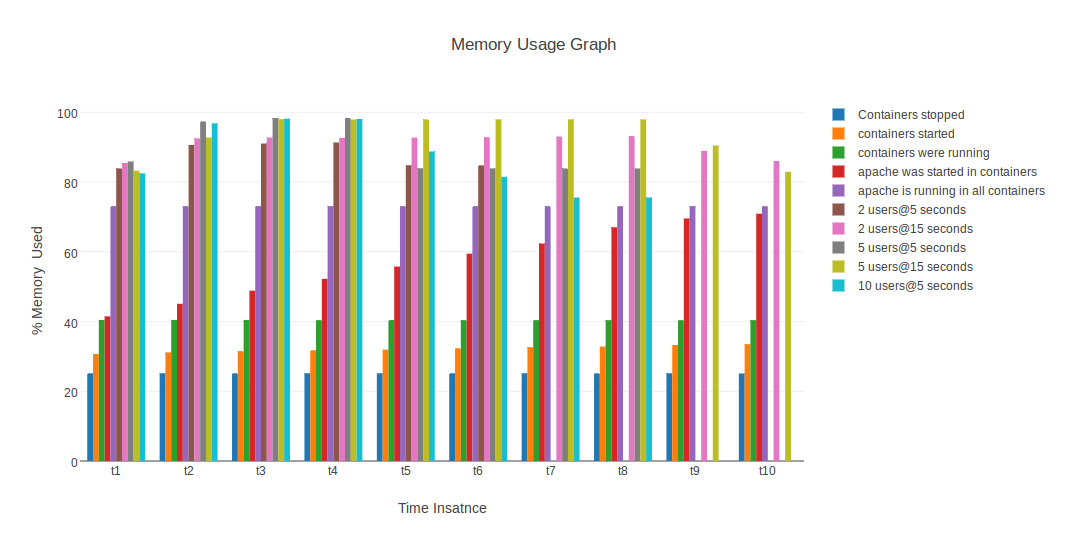
\includegraphics[width=.9\linewidth]{./images/memory-usage-time-bar-graph.png}
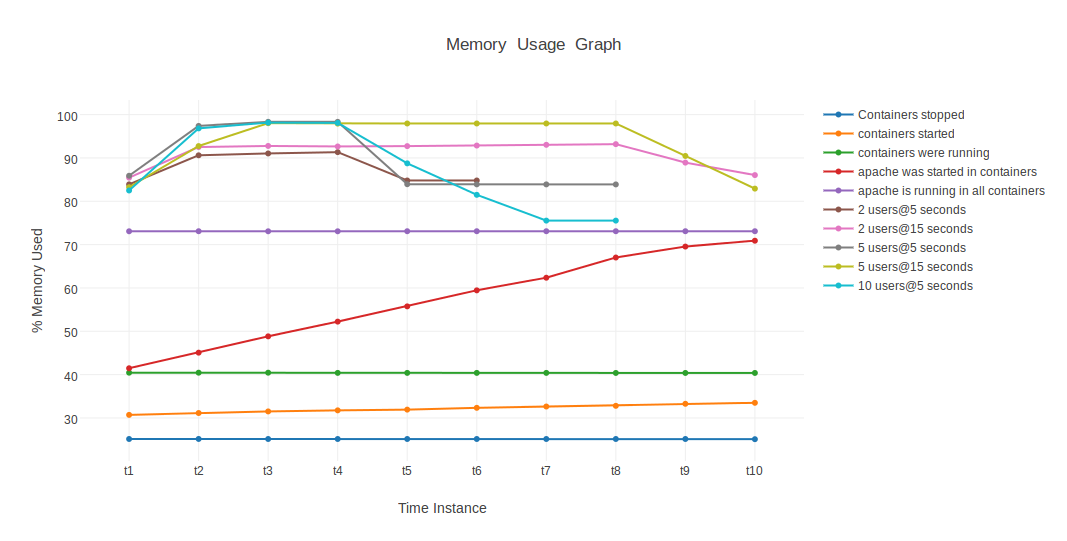
\includegraphics[width=.9\linewidth]{./images/memory-usage-time-line-graph.png}
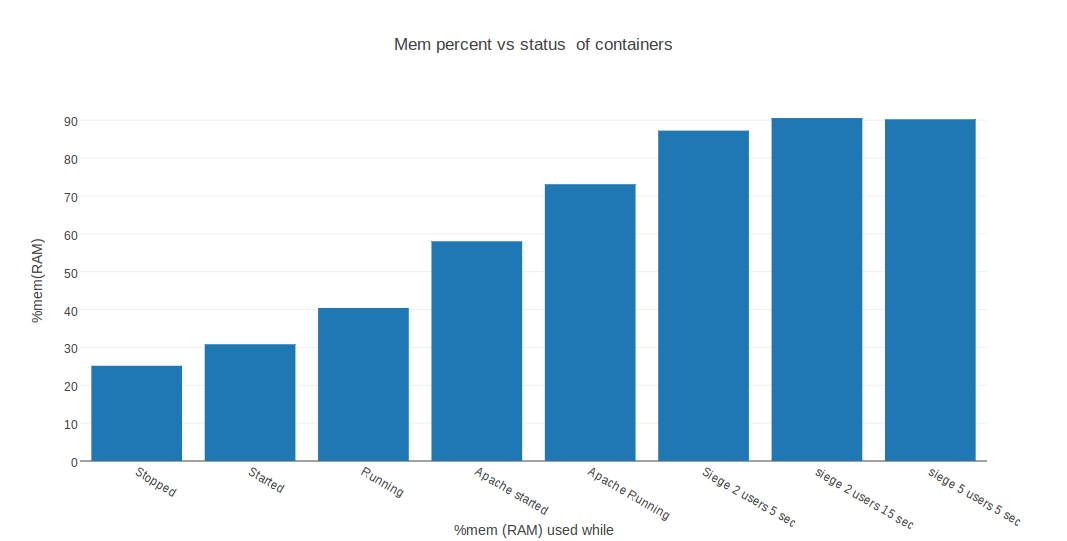
\includegraphics[width=.9\linewidth]{./images/memory-usage-container-status-bar-graph.png}
\end{itemize}
\subsection{Test using Fork bomb}
\label{sec:orgheadline49}
A fork bomb is a denial-of-service attack wherein a process continually
replicates itself to deplete available system resources, slowing down or
crashing the system due to resource starvation.
\begin{itemize}
\item \texttt{:()\{ :|: \& \};:}  This is fork bomb.
\item Due to this command you will run out of system resources and you may need
to reboot your system.
\item Here we tried to run fork bomb in one of the containers
\end{itemize}
\subsubsection{Testing Docker Container without limiting its memory}
\label{sec:orgheadline47}
\begin{itemize}
\item 1.Create and run a container :
\begin{verbatim}
$ docker run -it ubuntu:14.04 bash
root@ec164228902a:~# =:(){ :|: & };:
\end{verbatim}
\begin{itemize}
\item This container now will ask for more system resources from host
until you run of system resources.
\end{itemize}
\item 2.Since we ran out of resources, the host machine goes down and need to
be rebooted
\item 3.Thus we found out that the Docker container asks for system
resources from host when ever required without any limit.
Due to this if the container goes down it will crash the host.
\item 4.So we have to limit the memory usage of the container.
\end{itemize}

\subsubsection{Testing Docker container after limiting its memory}
\label{sec:orgheadline48}
\begin{itemize}
\item 1.Create and run a container(include memory limit)
\begin{verbatim}
$ docker run -it -m=200M ubuntu:14.04
root@ae164798902a:~# =:(){ :|: & };
\end{verbatim}
\item 2.This container will use memory of 200 MB only. If it asks for more than
200 MB then the container stop.
\item 3.To start the container again you have to use \texttt{docker start} command and
the container will start normally.
\item 4.Thus by limiting memory of a container, if any container crashes the
others will be still running normally
\end{itemize}
\section{Reference}
\label{sec:orgheadline51}
\begin{itemize}
\item Docker Tutorials -  \url{https://training.docker.com/self-paced-training}
\item Benefits of Docker - \url{https://access.redhat.com/documentation/en-US/Red_Hat_Enterprise_Linux/7/html/7.0_Release_Notes/sect-Red_Hat_Enterprise_Linux-7.0_Release_Notes-Linux_Containers_with_Docker_Format-Advantages_of_Using_Docker.html}
\item Docker Architecture - \url{https://docs.docker.com/v1.8/introduction/understanding-docker/}
\item Docker glossary -  \url{https://docs.docker.com/engine/reference/glossary/#union-file-system}
\item Docker Commands - \url{https://docs.docker.com/engine/reference/commandline/}
\item Docker file reference - \url{https://docs.docker.com/engine/reference/builder/}
\item Docker Data Volumes - \url{https://docs.docker.com/engine/tutorials/dockervolumes/}

\item Fork bomb -
\url{http://askubuntu.com/questions/159491/why-did-the-command-make-my-system-lag-so-badly-i-had-to-reboot}
\item Crontab - \url{http://www.adminschoice.com/crontab-quick-reference}
\item curl command - \url{https://curl.haxx.se/docs/manpage.html}
\item Load testing with siege -
\url{https://www.linode.com/docs/tools-reference/tools/load-testing-with-siege}
\end{itemize}
\end{document}
